\documentclass[a4paper,11pt]{article}
\usepackage[utf8x]{inputenc}
\usepackage[top=3cm,left=2.5cm,right=2.5cm,bottom=3cm]{geometry}
\usepackage[T1]{fontenc}
\usepackage[english]{babel}
\usepackage{graphicx}
\usepackage{amsmath}
\usepackage{amssymb}
\usepackage{setspace}
\usepackage{fancyhdr}
\usepackage{wrapfig}
\usepackage{subfig}
\usepackage{hyperref}
\usepackage{sidecap}
\usepackage{theorem}
\usepackage{thc}
\usepackage{url}
\usepackage{epsfig}
\usepackage{booktabs}
\usepackage{array}
\usepackage{multirow}
\usepackage{wrapfig}
\usepackage[floatrow]{chemstyle}
\usepackage{enumitem}
\usepackage{epstopdf}
\usepackage{multicol}
\usepackage{pbox}
\usepackage{cite}
\usepackage[compact]{titlesec}
\usepackage[makeroom]{cancel}
% ***********************************************************
% ******************* PHYSICS HEADER ************************
% ***********************************************************
% Version 2
%\usepackage{amsmath} % AMS Math Package
%\usepackage{amsthm} % Theorem Formatting
%\usepackage{amssymb}	% Math symbols such as \mathbb
\usepackage{graphicx} % Allows for eps images
\usepackage{multicol} % Allows for multiple columns
%\usepackage[dvips,letterpaper,margin=0.75in,bottom=0.5in]{geometry}
 % Sets margins and page size
%\pagestyle{empty} % Removes page numbers
%\makeatletter % Need for anything that contains an @ command 
%\renewcommand{\maketitle} % Redefine maketitle to conserve space
%{ \begingroup \vskip 10pt \begin{center} \large {\bf \@title}
%	\vskip 10pt \large \@author \hskip 20pt \@date \end{center}
 % \vskip 10pt \endgroup \setcounter{footnote}{0} }
\makeatother % End of region containing @ commands
\renewcommand{\labelenumi}{(\alph{enumi})} % Use letters for enumerate
% \DeclareMathOperator{\Sample}{Sample}
\let\vaccent=\v % rename builtin command \v{} to \vaccent{}
\renewcommand{\v}[1]{\ensuremath{\mathbf{#1}}} % for vectors
\newcommand{\gv}[1]{\ensuremath{\mbox{\boldmath$ #1 $}}} 
% for vectors of Greek letters
\newcommand{\uv}[1]{\ensuremath{\mathbf{\hat{#1}}}} % for unit vector
\newcommand{\abs}[1]{\left| #1 \right|} % for absolute value
\newcommand{\avg}[1]{\left< #1 \right>} % for average
\let\underdot=\d % rename builtin command \d{} to \underdot{}
\renewcommand{\d}[2]{\frac{d #1}{d #2}} % for derivatives
\newcommand{\dd}[2]{\frac{d^2 #1}{d #2^2}} % for double derivatives
\newcommand{\pd}[2]{\frac{\partial #1}{\partial #2}} 
% for partial derivatives
\newcommand{\pdd}[2]{\frac{\partial^2 #1}{\partial #2^2}} 
% for double partial derivatives
\newcommand{\pdc}[3]{\left( \frac{\partial #1}{\partial #2}
 \right)_{#3}} % for thermodynamic partial derivatives
\newcommand{\ket}[1]{\left| #1 \right>} % for Dirac bras
\newcommand{\bra}[1]{\left< #1 \right|} % for Dirac kets
\newcommand{\braket}[2]{\left< #1 \vphantom{#2} \right|
 \left. #2 \vphantom{#1} \right>} % for Dirac brackets
\newcommand{\matrixel}[3]{\left< #1 \vphantom{#2#3} \right|
 #2 \left| #3 \vphantom{#1#2} \right>} % for Dirac matrix elements
\newcommand{\grad}[1]{\gv{\nabla} #1} % for gradient
\let\divsymb=\div % rename builtin command \div to \divsymb
\renewcommand{\div}[1]{\gv{\nabla} \cdot #1} % for divergence
\newcommand{\curl}[1]{\gv{\nabla} \times #1} % for curl
\let\baraccent=\= % rename builtin command \= to \baraccent
\renewcommand{\=}[1]{\stackrel{#1}{=}} % for putting numbers above =
\newtheorem{prop}{Proposition}
\newtheorem{thm}{Theorem}[section]
\newtheorem{lem}[thm]{Lemma}

% ***********************************************************
% ********************** END HEADER *************************
% ***********************************************************
\usepackage{indentfirst}
\usepackage[toc,page]{appendix}



\long\def\symbolfootnote[#1]#2{\begingroup%
\def\thefootnote{\fnsymbol{footnote}}\footnote[#1]{#2}\endgroup}

\geometry{ bottom=2 cm}


\setlength{\abovecaptionskip}{-10pt plus 3pt minus 2pt}


\setlength{\headheight}{15pt}

\fancyhf{}
\fancyhead[RO,LE]{\footnotesize{\leftmark}}
\fancyhead[LO,RE]{\thepage}

\pagestyle{fancy}

\renewcommand\maketitle{
\begin{titlepage}

 \begin{center}
 \begin{figure}[htpb]
\rule{1 \textwidth}{1pt}\\
 \smallskip  
 \end{figure}

\vfill

\textbf{ \begin{huge}
Developing a Predator-Prey Simulation
\end{huge}}

\vspace{0.4cm}

\begin{Large}
 \textit{Programming Skills Group Report}
\end{Large}

\vspace{1cm}


\begin{tabular}{ccc}
\large{Diamantis Ntakaris, Ewen Lawson Gillies, Michal Kawalec, Claude Schmidt} \vspace{0.15cm}\\
\large{\textit{University of Edinburgh, UK}}\\
\end{tabular}




  
\vspace{0.7cm}
\vspace{0.7cm}

\includegraphics[width=0.33\textwidth]{edinburgh_crest.jpg}\\
\vspace{0.7cm}
\Large{7th of November 2013}

\end{center}

\vfill

\begin{abstract}

The aim of this project is to develop the essential programming skills through developing a predatory-prey simulation.  The group was given a system of coupled partial differential equations that the population densities of pumas and hares on a 2D surface.  Using \texttt{C++} and other existing programming frame work, an efficient, portable, and extendable simulation was developed.  This simulation was then throughly tested, debugged, and optimized.  Despite being a relatively simple simulation, the analysis was able to give insight into the dynamics of the problem.

\end{abstract}


\vfill


  \begin{center}
 \rule{1 \textwidth}{1pt}\\
 \end{center}



\end{titlepage}}

\begin{document}

\maketitle
\tableofcontents
\newpage
\setcounter{page}{1}



\section{Introduction}
The focus of this project was to apply the skills acquired in class to develop a Predator-Prey simulation in a group setting.  This group opted write the program in \texttt{C++}.  In order to do so, the project members started with a rough outline of the program.  From here, development tasks were assigned to each member.  The revision control software $\texttt{git}$ was used to streamline the collaborative efforts of the group.  Once a working simulation was written, it was thoroughly tested, debugged, and improved.  The resulting simulation includes several output types for different visualization programs.  

For reference, the coupled partial differential equations that dictate the time evolution of the populations of pumas and hares are included below.  $H$ is the population of hares, $P$ is the population of pumas, $x,y,$ and $t$ are space and time coordinates respectively, and $r,a,k,b,m$ and $l$ are scaling parameters, as discussion in Section \ref{params}.

\begin{equation}\label{hares}
\pd{H}{t} = rH - aHP +k\left(\pdd{H}{x} + \pdd{H}{y}\right)
\end{equation}

\begin{equation}\label{pumas}
\pd{P}{t} = bHP - mP +l\left(\pdd{P}{x} + \pdd{P}{y}\right)
\end{equation}

\section{Group Coordination}

As with any software development, the planning played a big role in the final product.  Through regular meetings, emails, task management websites, and revision control repositories, plans were set and efforts were coordinated to ensure an efficient and productive group effort.  

\subsection{Group Members Responsibilities}

In order to increase efficiency and productivity, the division of labour was determined very early on.  This division was based primarily on the existing skills set of each member.  Each member was mandated to some of the coding. The more experienced coders edited the work of the less experienced once in a hierarchical order. The most experienced then explained his reasoning to the rest of the group, giving them an opportunity for further input into the final code.  This ensured both an optimal simulation, learning experience, and supportive feedback for each member.  The breakdown of the tasks and responsibilities for each member in order of coding previous experience in $\texttt{C++}$ are as follows.
\\

\noindent\textbf{Michal Kawalec:}  Due to his experience in software development and project management, Michal set up the structure of the simulation and submitted this structure to a repository on \url{https://github.com/mkawalec/pumas}.  This structure included the header files and source files appropriately formatted with empty functions as well as the build system configuration. Michal also conducted all final edits, adapting the other members ideas to the optimal syntax.
\\

\noindent\textbf{Claude  Schmit:}   With a strong working understanding of $\texttt{C++}$, Claude was tasked with writing the first draft of the constructor. Once the main simulation was set up, he extended the test framework and included various sanity checks into the test-suite. After moving to a more advanced output structure, Claude was tasked to implement the \texttt{PlainPPMSerializer} and its dependencies. Having a first working version, it was his job to create various landmaps on which he then ran the simulation. He also provided the group with the structure and planning needed for optimal time management.  
\\

\noindent{\textbf{Ewen Gillies:}  Given his experience in numerical solutions to partial differential equations, Ewen was tasked with writing the integrating function and dealing with the boundary cells.  Since he lacked experience in $\texttt{C++}$, any additional structural ideas ideas were relayed to the more experience coders for optimal syntax.  He then reviewed this code to ensure all ideas were properly expressed.  Additionally, he was tasked with compiling the group report.
\\

\noindent{\textbf{Diamantis Ntakaris:}}  Using his strong mathematical background, Diamantis conducted the preliminary analysis of the equation at hand, as well as the intermediate and final analysis of the output.  He also wrote the initial output function, which was then extrapolated to the final one.  As a relatively inexperienced coder, Diamantis was able to offer effective continual feedback on readability and the logical structure of the code, ensuring that all levels of coders would be able to read code and reproduce the results.  He also generated several of the input land maps for the simulation.

\subsection{Coordination}

The main method of group coordination and planning was through regular meetings.  
Full group meetings were held at least once per week, where new ideas and current progress could be discussed.  
During these meetings, smaller meetings between two or three members were organized where code would be peer edited or written by several members at once.

The members of the group agreed to use \texttt{Trello}\footnote{This tool is found at: \url{https://www.trello.com}} in order to ensure flexibility in task assignment and adaptability in the testing and debugging phases.  
This tool consists of four communal lists that each person can edit.  
These lists include \emph{To Do, Review, Doing,} and \emph{Done. }
By adding items to the to do list, shifting them to doing, and placing them in done, group efforts were easily and effective coordinated without any overlap.

\section{Design} 

This simulation has three major comments: Input, Simulation, and Output.  
It is designed to accept an ASCII file that determines the land map of the simulation.
The parameters that dictate the time evolution of the hare and puma populations can also be adjusted, although default values are provided.  
The simulation is then initialized, run for a set amount of time steps, and properly finalised.  
A a regular interval of time steps, the population of hares and pumas is printed to an output file using one of the available output methods.  
These outputs can then be visualized, plotted, and analyzed.

\subsection{Input}

The simulation must read in an input land map.  
This land map represents the two dimensional surface on which the simulation takes place.  
This surface can either be land, where hare and puma populations are allowed, or water, where they do not exist.  
The user has the option of setting the parameters that dictate the dynamics of the system as well, although default values are automatically provided.  
The land map and all input parameters are initially parsed by \texttt{solver.cpp}.

\subsubsection{Parameters}\label{params}

The input parameters can be set by the user, otherwise the default values are automatically initialized.  
These parameters are divided into four categories: generic options, simulation parameters, simulation options, and input/output options.
The generic options include displaying a help menu and the version of the simulation.  
The simulation parameters include the scaling factors of the terms in the coupled partial differential equations \eqref{hares} and \eqref{pumas}.  
The simulation options include the size of the time step, the frequency of the output, and the time at which the simulation ends.  
The input/output options include the output names, extensions, and formats as well as the frequency at which the progress of the simulation is printed to the terminal.  

All of the parameters are set using the \texttt{boost/program\_options} library, using the traditional syntax. 
See Appendix~\ref{syntax} for an example.~\ref{tb:parameters}, below, contains a list of the simulation parameters and their default values. 
Note that shorthand parameters can be combined, so parameter \texttt{-oa output} is a valid sequence.

Parameter sets other than the Generic options can be set from a configuration file. 
This format uses the same parameter names as the command line, with a slightly different syntax. 
For an example, please see the \texttt{contrib/example.cfg} in the supporting documents.

\begin{table}
\centering
\begin{tabular}{|l|l|l|l|}
\hline
\textbf{Type} & \textbf{Name} & \textbf{Description} & \textbf{Default} \\ \hline
\multirow{2}{*}{\pbox{10cm}{Generic \\ Options}}
 & \texttt{-h, -{}-help} & Show help message & N/A \\
 & \texttt{-v, -{}-version} & Show program version & N/A \\ \hline
\multirow{6}{*}{\pbox{10cm}{Simulation \\ Parameters}} 
 & \texttt{-r, -{}-r} & Birth rate of hares & 0.08 \\
 & \texttt{-a, -{}-a} & Rate at which pumas eat hares & 0.04\\
 & \texttt{-b, -{}-b} & Birth rate of pumas per hare eaten & 0.02 \\
 & \texttt{-m, -{}-m} & Mortality rate of pumas & 0.06 \\ 
 & \texttt{-k, -{}-k} & Diffusion rate of hares  & 0.2 \\ 
 & \texttt{-l, -{}-l} & Diffusion rate of pumas & 0.2 \\ \hline
\multirow{3}{*}{\pbox{10cm}{Simulation \\ Options}} 
 & \texttt{-e, -{}-end-time} & End time & 1000 \\
 & \texttt{-{}-dt} & Time step & 0.01\\
 & \texttt{-p, -{}-print-every} & Iterations between output frames & 100\\ \hline
 \multirow{7}{*}{\pbox{10cm}{\ \\ \ \\ \ \\ Input/Output \\ Options}} 
 & \texttt{-d, -{}-data-file} & Location of parameters file & none \\
 & \texttt{-o, -{}-output} & Filename of the main output file & \texttt{output} \\
 & \texttt{-u, -{}-aux} & Filename of the auxiliary output file & none \\
 & \texttt{-f, -{}-output-format}  &  Format of the output& \texttt{vmd} \\
  & &  (\texttt{vmd, gnuplot, ppm})   &  \\ 
 & \texttt{-x, -{}-output-extension} & Overrides the output extension & none \\
 & \texttt{-n, -{}-notify-after} & Output frames between printing  & 30 \\
  & & progress to terminal.  &  \\ 
 & \texttt{--split-files} & Forces the serializer to print each & \texttt{false} \\ 
 & & time frame to a new file.  &  \\ \hline

\end{tabular}
\caption{A table of input parameters and their default values.}
\label{tb:parameters}
\end{table}


\subsubsection{Land Map}

The surface is discretised to have an $x$ and $y$ dimension, denoted interchangeably as \texttt{size\_x}, \texttt{dim\_x} and \texttt{size\_y}, \texttt{dim\_y}.  These two parameters are defined in the first line of every land map input file, and read in during the \texttt{ PUMA::Simulator* initialize} function in \texttt{solver.cpp}.  The rest of the land map input file entries are either 1 or 0 to denoted land or water.  To ensure the file format reflects the geometry of the surface, each line has \texttt{size\_x} entires, while the whole file has \texttt{size\_y} lines. The land map is read into the program at start up by naming it in the terminal, as shown in Appendix \ref{syntax}.

These file maps can be generated in any way that respects the description above.  The ones included in the submission were generated using \texttt{Gimp}\footnote{This freely distributed software is available here: \url{http://www.gimp.org}}.  The advantage of using this program is it allows the user to draw the desired land map in black and white, and then outputs this file to a portable anymap (PNM) format.  This file is then transferred to the desired \texttt{ASCII} format using the \texttt{pnm2dat} program.  Likewise, arbitrary image files can be opened, changed to black and white, and outputted to the desired land map format.

\subsection{Simulation}

The structure of the simulation itself is straightforward.  \texttt{Simulator.cpp} contains the majority of the computation and simulation properties.  The \texttt{solver.cpp} file contains the main function, along with an input parameters parser and \texttt{Simulator} class instantiation.  The results of the simulation passed to \texttt{Serializer.cpp} for printing.  These results can then be visualized.  For more on in-depth discussion of output, see Section \ref{output}.

\subsubsection{Initialization}

The simulation starts by parsing all input parameters and the land map file in the \texttt{solver.cpp} class.  First, the land map input file accessed by the \texttt{initialize} function.  As per the input file format, the first two entires are used to define the dimensions of the simulation .  The rest of the entries are stored in the one dimensional boolean \texttt{land\_map} array which has ($\texttt{dim\_x} \times \texttt{dim\_y}$) elements.  In this array, a value of \texttt{true} corresponds to a land entry, whereas \texttt{false} corresponds to a water entry.  The function then constructs a \texttt{Simulator}, as defined in the \texttt{Simulator.cpp} file, with the appropriate dimensions and land/water entries.  

\subsubsection{Construction}

The \texttt{Simulator} constructor effectively starts by allocating enough memory for store the information of two subsequent time steps.  These states are  referred to as \texttt{current\_state} and \texttt{temp\_state}.  Using the \texttt{boost} library, they each defined as a \texttt{shared\_array}\footnote{See section (REF) for a discussion of \texttt{shared\_arrays}}} of \texttt{landscape} entries.  The \texttt{landscape} structure\footnote{This structure is defined in \texttt{\textbackslash include\textbackslash helper.hpp}} stores information about the cell including whether it is land or water, the hare population, and the puma population. The boolean \texttt{land\_map} array is copied on to both states.  The land cells in the \texttt{current\_state} are then given a random\footnote{The random number generator is seeded according to the start time to ensure unique results for each run.} population of hares and pumas between 0 and 5, whereas the water cells are set to 0.  All cells in the \texttt{temp\_state} are initialized to zero.

The simulation is built with default values for all parameters.  After the constructor is called, the \texttt{solver.cpp} class reads any user set values and sets the simulator values accordingly, including the output type.

\subsubsection{Calculation}

After declaring some output streams and initializing an \texttt{average\_densities} structure\footnote{This structure stores one double for average hare density and one for average puma density, as defined in \texttt{\textbackslash include\textbackslash helper.hpp}.}, the simulation moves into the main calculation loop.  This loop is defined to iterate the simulation from the initial time to the final time in the defined time-step increments.  Most of the work is done in the \texttt{apply\_step} function, as defined in \texttt{Simulator.cpp}.  

The  \texttt{apply\_step} function starts by switching the contents of the  \texttt{current\_state} and the \texttt{temp\_state}.  It then opens a loop through all the sites in the system.  If the site is a land cell, it counts the number of neighboring land cells for use in the discretized partial differential equations.  The values in \texttt{temp\_state} are used to calculate the updated populations according to equations \eqref{hares} and \eqref{pumas} (REF), which are then stored in \texttt{current\_state}.  These values have a minimum value of zero.  All water cells are skipped so that their populations remain at zero.
.  

A key part of the \texttt{apply\_step} function is that it accesses all cells through the \texttt{get\_cell} function.  For all defined cells on the map, it returns the value of the \texttt{temp\_state}, as expected.  For all cells outside the limits of the system, it returns the \texttt{halo\_cell} which was initialized in the constructor.  Since all cells outside the system are defined to have a zero population, this is a cost effective way of setting and changing the boundary conditions.

% In a sense yes, but the main point of get_cell is that it enables 
% very easy change in the boundary conditions - you just change the
% get_cell proxy. The space savings are diminishing with increasing
% map size, in in the UK case we are saving just 0.1%

After the system is moved forward one time step, the average populations across all land cells are calculated.  These averages are printed to the terminal every \texttt{n} frames with the total data passed to the serializer every \texttt{p} frames, as defined in \ref{tb:parameters}.

\subsection{Output}\label{output}

The output of the simulation is handled by the \texttt{Serializer.cpp} file.  This file defines three output formats, each with its own class.  One format is chosen as a parameter of the current simulation.  The main loop tells the \texttt{Simulator.cpp} class to print, which then passes all the information to the \texttt{Serializer.cpp} where it is properly formatted.   This is intended to maximize flexibility in adding, removing, and choosing available output formats.  Once the output file has been generated, it can be visualized using one of several visualizers.

\subsubsection{Serializer}

\texttt{Serializer.cpp} is designed to effectively handle the output file format and nothing else.  It defines a class for all available output format.  These classes are all named and pointed to using a list of pointers.  \texttt{Simulator.cpp} defines a pointer to a \texttt{Serializer.cpp} class called \texttt{current\_serializer}.  Strictly speaking, the simulator is initialized as pointing to nothing.  It is then set to point to the desired format class in \texttt{solver.cpp} via the \texttt{choose\_output\_method(}\emph{arg}\texttt{)} function.  This function checks its argument against the names of the formats pointed to in the list, returning the appropriate pointer in the event of a match.  If none match, then the program returns an error.  In the event that the function is never called, \texttt{Simulator.cpp} sets \texttt{current\_serializer} to point to the first pointer of the list of available serializers.  

Once the  \texttt{current\_serializer} is set, \texttt{Simulator.cpp}  knows to where pass all the output data.  In the main loop, \texttt{solver.cpp}  opens two out streams, which are then passed to the \texttt{Simulator::serialize} function.  This function passes these out streams, as well as the \texttt{current\_state} and dimensions of the system to the address of the \texttt{current\_serializer} pointer, which is a class defined in \texttt{Serializer.cpp}.  This class then handles all formatting, and prints the contents of the current state to the appropriate stream.

For the purposes of this simple simulation, this output method is over engineered.  Its true strength and simplicity is only realized when the simulation has more than one output type.  By including \texttt{Serializer.cpp}, the output method is adaptable, scaleable, and separates concerns.  Should a new format be needed, only \texttt{Serializer.cpp} and its header file need to be edited.  The motivation to include several output types was to test the outputs using several visualization methods.

\subsubsection{Visualisation}\label{visual}

A key part of any simulation is the ability to visualize the results.  This program has been configured to output file types usable for three visualization program.  These visualizers are \texttt{Visual Molecular Dynamics, Gnuplot} and \texttt{Imagemagick}, the last of which is used to visualize PPM files.  Each of these programs have their strengths and weaknesses, as discussed below.  Links to sample visualizations are provided in Appendix \ref{links}.

The most informative of the three is \texttt{Visual Molecular Dynamics, VMD}.  While this visualizer is intended to model molecule interactions, it accepts an \texttt{XYZ} file type, where the location of each particle is written in Cartesian coordinates for every time step.  The populations of pumas and hares can be stored as the $z$ coordinate of a ``particle,'' with the $x$ and $y$ coordinates representing which cell they are in.  The main advantage of this visualizer is that it allows for a 3D visualization of the data.  This visualization can then be rendered to a video file format, which is both compact and portable.  The disadvantage is that it is computationally intense to process large maps and render high quality videos.  

The easiest viewer is \texttt{Gnuplot}.  This visualizer offered the most flexibility in visualization options using a relatively easy script.  A \texttt{Gnuplot} script is used to generate a color map to plot the populations against $x$ and $y$ at every time step.  These maps are then strung together in a \texttt{gif}.  The advantage of this visualizer is that is is the only one that includes a quantitative colour scale for the populations, as well as an indication of the current time step.  The downside to this viewer is that it takes a very long time to load large data files and requirers \texttt{Gnuplot} to be installed.

The most portable visualization is when the populations are printed directly to a Portable Pixmap (PPM) format.  This generates image files directly from the \texttt{Serializer}, which are readable by nearly all systems and imaging processing software.  These files were processed by \texttt{imagemagick} to create a \texttt{.gif} moving image.  The difficulty with this output is that it is difficult to recover any kind of scale from the resulting images.  The only conclusive evidence they offer is whether or not a steady state is reached.  



\section{Tools and Frameworks}

The simulation was written in \texttt{C++}, which had a large impact on the tools and frameworks used throughout the project.  The code was compiled with \texttt{gcc} version 4.8.  The unit testing framework, as well as several key features, were included from the \texttt{Boost} library.  \texttt{Cmake} was used to help generate \texttt{Makefiles} across several different platforms.  From there, \texttt{gdb} was used to help debug the program.  Once the program was running, the performance testing tool \texttt{Valgrind} was used in order to optimize the code.  Finally, all documentation was was generated using \texttt{Doxygen}.

\subsection{Programming Language}

\texttt{C++11} was the primary programming language used to write this simulation.  This is the most current version of \texttt{C++}.  Using this programming language, the simulation is designed to be  reusable, extendable, and self contained. In order to do so, it utilizes a main function that calls upon methods contained in independent library\footnote{These files are not a formal \texttt{C++} ``library,'' but do behave like one.}.  This library can easily be utilized by a different main function with equal success.  A new simulator obeying a different partial differential equation can be produced inheriting from a \texttt{Simulator} class and overloading the \texttt{apply\_step} function.  Likewise, the boundary conditions are easily changed by overloading the \texttt{get\_cell} function.  In order to ensure there are no clashes with existing libraries, the simulator defines its own namespace, \texttt{PUMA}.   

\subsubsection{Complier}

The simulation was compiled with \texttt{gcc} version 4.6, which is the most widely available version on current \texttt{Linux} distributions.  This is to ensure that the program can run on many platforms.  Unfortunately, only the features of \texttt{C++11} implemented in this version of \texttt{gcc} were used.  For example, the newer version of \texttt{gcc}, version 4.8, supports constructor inheritance, which would have been useful in defining the constructors in \texttt{exceptions.hpp}.  Instead, a constructor and destructor needed to be defined for each exception. 

%SOMETHING ELSE

\subsubsection{Boost}

\texttt{Boost} is one of the most widely used, reviewed, and tested \texttt{C++} libraries.  It greatly improved the memory management, parsing methods, and standard functions  available to the simulation.   It also provided a unit testing framework, as discussed in Section \ref{test}.  

To improve memory management, \texttt{boost::shared\_array} was used.  This object is an instance of a \emph{smart pointer}.  Smart pointers ensure that an object is automatically removed from memory once all references to that object go out of scope.  This is to say that once all smart pointers to an object are no longer available to the simulation, this object is removed from memory.  This property is especially useful when dealing with the large arrays found in \texttt{Simulator.cpp}.  
%Additionally, the \texttt{swap} function of the \texttt{shared\_array} was very useful in the \texttt{apply\_step} function.  This function swaps the address of two 

Using \texttt{Boost}, the program options can be defined, grouped, and easily set at runtime.  This library also enables configuration files to be used with little added code.  The program options are also conveniently stored and displayed in a help menu, which can also be displayed at runtime.  

Finally, the \texttt{Boost} was used to define a Mersenne-Twister random number generator.  This random number generator is seeded with the current time up to a microsecond.  This is to ensure a unique seed for all simulator classes, even when they are instantiated within a small time frame.  The advantage of using the Mersenne-Twister generator is that it has been proved to have a better random number distribution and a longer period than the standard \texttt{C++} random number generator.  Additionally, it is widely used, and has been throughly tested.

\subsection{Build}

In order to build the simulation, a \texttt{Makefile} must be generated.  \texttt{CMake} was used to abstract this process, ensuring that it is as system independent as possible.   This is done using \texttt{find} scripts, which only require the user to supply the names the needed include files.  The paths to these files are determined, and printed to the \texttt{Makefile}.  Additionally, \texttt{CMake} prints the the build process, detailing the progress and any errors.  The disadvantage is that it requires the installation of the latest version of \texttt{CMake}, which is not available on Scientific Linux/  

\subsection{Revision Control}

The revision control software \texttt{git} was used to streamline group editing of the source code and coordinate efforts between group members.  This software based on a decentralized repository structure, which is favorable to a centralized repository structure.  By decentralizing, the development no longer has a single point of failure.  In addition, decentralized structures allow for easy write privilege management and allow changes can be committed offline.

\texttt{git} was chosen over the popular decentralized alternatives because it is the mostly widely supported and fasted available.  Using \texttt{git} meant that the free online repository \texttt{GitHub} could be used.  Using this software, changes could be tracked and visualized.  It was one of the most important lines of communication between group members.


\subsection{Testing}\label{test}

All unit testing was done with \texttt{boost::UNIT\_TEST}.  This library is included in \texttt{boost} and provides the basic functionality needed for the program.  Tests were included in a \texttt{test\_suite.cpp} file.  The first of these tests ensure that the simulator can be constructed and that the land map is parsed correctly.  The next set ensures that the \texttt{apply\_step} function effects the populations of the land cells, but do not effect the populations of the water cells.  To test the output, the \texttt{test\_suite} turns off all birth and death rate terms to ensure the diffusion of populations works correctly.   

Performance profiling was used to optimize the simulation.  This profiling was done with \texttt{Valgrind} using the \texttt{Callgrind} tool.  This tool provided an estimate of the time spent on each function. The performance profiling reveal that 94.11\% of the computation was devoted to printing the output, with only 0.861\% spent on the actual \texttt{apply\_step} calculation.  This motivated the group to decrease the default time step and print frequency by a factor of 100.  After this optimization, 64.34\% was spent on printing, with 33.83 \% spent on calculations.  This greatly improved the accuracy of the simulation without significantly increasing the computation time.  The \texttt{Kcachegrind} tool visualized this information.  See Appendix \ref{Kcashegrind} for an example of this output. 

\subsection{Debugging}

The simulation was debugged using \texttt{gdb}.  In order to do so, the program was compiled with the \texttt{-g} flag.  By setting break points, the components simulation were compartmentalized so that sources of error could found.  For example, the \texttt{halo\_cell} structure was not properly instantiated the first time.  A break point allowed the group to review the contents of the cell before the program crashed, revealing this error.   

To ensure that there were no memory leaks in the program, the \texttt{memcheck} tool from \texttt{Valgrind} was used.  This tool revealed that boolean \texttt{land\_map} array was not destructed after it had been parsed to \texttt{current\_state} and \texttt{temp\_state}.  
 
 \subsection{Documentation}

In order to document our code, we opted for the \texttt{Doxygen}\footnote{See \url{http://www.doxygen.org} for details.} documentation generator. This tool reads the source files and generates documentation according to the comments inside the \texttt{C++} code, as long as these follow the necessary syntax. \texttt{Doxygen} then creates the documentation in various output formats. One such output is an easy to navigate \texttt{html} page that is readable by most web-browsers. It also provides a \LaTeX \ script that can be run to produce a concise user manual. The resulting documentation shows the class structure that is used in the source code as well as a description of all functions, structures, and variables used. The use of \texttt{Doxygen} allowed us to focus on producing a working product without having to worry about also writing documentation, as we could readily produce this as a side product by sensible commenting.   
 
 \section{Analysis}
 
 
Once the simulation was running, several maps were tested with different time steps.  These runs were visualized using the methods discussed in Section \ref{visual}.  By visualizing the results, the group was able to spot some weaknesses in the code very early on.  Once these weaknesses were fixed, the resulting simulations were analyzed to determined some qualitative properties of the system.

\subsection{Instabilities}

One of the earlier visualizations showed a diverging behaviour in the populations, where the amplitude increased with every oscillation.  This caused negative populations to occur, which destabilized the system.  The average population of this simulation is shown in \ref{fig:unstable}.  Following this result, the time step was lowered and the populations were given a minimum value of zero.  This stabilized the simulation.  These two comparative visualisations are linked in Appendix \ref{links}, with titles ``Unstable'' and ``Stable'' respectively. 

\begin{figure}[h]
\includegraphics[width=\textwidth]{unstable.eps}
\caption{Unstabile Average Population}
\label{fig:unstable}
\end{figure}
 

\subsection{Average Densities} 
Once the code was stabilized, the average populations were mapped against time.  The plot below in \ref{fig:stable} shows the average population of pumas and hares across a 2000$\times$2000 map with the default settings.  It is clear from this plot that both average population are sinusoidal and in a dynamic equilibrium.  With these parameters, the hares almost always have a higher population than the pumas, except for a brief period once per cycle.  
 
\begin{figure}[h]
\includegraphics[width=\textwidth]{stable.eps}
\caption{StabileAverage Population}
\label{fig:stable}
\end{figure}
 
 
Upon close inspection, it seems that the concavity of the puma population is related to the slope of the hare population.  This is to say that as the hare population diminishes or increase, the acceleration of the puma population likewise diminishes or increases.  This is an understandable result, since the total number of pumas births depends on the availability of hares.  Once the total number of pumas born per time step is very high, they eat more hares than normal, and the hare population plummets.  As it does so, the rate of puma birth deceases, and the cycle continues.  This relationship is the foundation of the dynamic equilibrium achieved.  It is clearly expressed in equations \eqref{hares} and \eqref{pumas}, and unsurprisingly reflected in the result.  This qualitative analysis implies that the simulation is accuracy. 

\subsection{Population Surface Features}
 
It is clear from the source code and from the visualization that the initial populations are entirely random.  This causes the population from cell to cell to be discontinuous.  Using any of the three visualization types, it is clear that this discontinuity is quickly smoothed out, on the order of a quarter of the period of population oscillation.  The random distribution still causes features in the population surface to persist.  As time passes, these features lessen, until the population surface becomes flat.  This behaviour is due to the diffusion terms equations \eqref{hares} and \eqref{pumas}.  This result implies that these diffusion terms act somewhat independently to the birth, death, and predation terms.  For links to these visualizations, see Appendix \ref{links}.
 
\section{Further Works}

The finished simulation, documentation, and analysis were all to the groups satisfaction.  With that said, several ideas were never properly implemented due to time constraints.  These included introducing different dynamics and initial conditions to the simulation, as well as expanding the output options.  The following section details some of these ideas.

\subsection{Novel Dynamics}

The partial differential equations and random initial condtions that dictated the dynamics of the system represent one of the simplest Predator-Prey simulations.  The easiest extension to this simulation would be to introduce new initial conditions.  It was suggested that these conditions could introduce dense pockets of hares an pumas that do not touch at first on different locations on the map or surround a low population of pumas with lots of hares  and observe the result.  An analysis of how the initial conditions effect the final out come has the potential to add a substantial amount of content to the simulation.  

Perhaps a less obvious extension that was suggested would be to have both populations prefer to be close to water sources.  The two hypothesized methods of achieving there were to introduce new terms to equations \eqref{hares} and \eqref{pumas} or to make the birth and death rate constants functions of the the distance from water.  While the exact effects could only be speculated, this feature does reflect real Predator-Prey simulations.  It has the potential to completely change the dynamics of the system, and would have been interesting to explore

\subsection{Improved Output}

A lot of the work done on this project focused on including a wide range of outputs.  Since the majority of this work was not prompted by the project description, the focus was on the ensuring that the infrastructure that provided the output was optimal.  This meant that once an output/visualization pair was working, efforts were shifted to less developed parts of the simulation.  As a result, the output files and/or visualizations produced are not optimal.  

The \texttt{VMD} output populates three ``molecules'' per cell, one for hare population, one for puma population, and one for land/water, regardless of cell type.  This means that each water cell has two more molecules than needed, since we know the populations in these cells are always zero.  These two extra cells cause the the output file type to be larger than needed and result in an ambiguous colour scheme in the final visualization.  Were there more time, the land map would be pre-scanned before serialization, and each water cell would only be given one molecule.

The \texttt{Gnuplot} output is informative, compact, easy to use, and fairly portable.  It provides useful visualizations of the populations vs. position using a 2D color map.   \texttt{Gnuplot} also supports 3D contour maps to the same data.  Additionally, the color of these contours can be used to plot a fourth variable.  Adding this feature to the list of available visualizers would have been fairly straight forward, and very powerful.  

Finally, the \texttt{PPM} output fails to show any kind of scale in its visualizations.  While it is useful for to ensure the simulation has not destabilized and to get a rough, qualitative sense of the dynamics, it fails to show exactly what range the populations are in.  Adding a color scale, either as a separate image file or in the same image file as the visualization would drastically improve the utility of these visualizations.
 
 \section{Conclusion}

The members were able to coordinate their efforts to plan, write, develop, debug, and optimize a basic Predator-Prety simulation.  Through a group effort, each member was able to contribute to the areas they were comfortable with, while learning more about the areas they were less familiar with.   The combined result is a well functioning, portable, efficient,   simulation.  While the simulation itself is quite simple, the structure is designed to be extended to more complex scenarios.  Despite its simplicity, the output of the simulation provided a qualitative insight to the dynamics of the system.  Were there more time, further analysis could have been done involving different initial conditions and novel dynamic variables.  While all the output methods are in working order, each has plenty of room for improvement.  Overall, this project has been a huge success.  The group was able to work as a team at every point of the process to produce a high quality final product. 

\newpage
\begin{appendices}
\section{Quick Start Guide for Simulation }
\subsection{Creating Input Land Maps}

To create input land maps, open the \texttt{puma/data/} directory and and run \texttt{gimp} version 2.8. Select \texttt{File $\rightarrow$ New} and enter the size of the desired land map in the window that opens.  Be sure to select \texttt{Greyscale} under \texttt{Advanced Options} and then press \texttt{OK}. An interface will open where the land map can be drawn. Note that points lighter than \texttt{greyscale} = 128 will be water, whereas the darker ones will be land. Once the map is drawn, select \texttt{File $\rightarrow$ Save as} and enter the desired file when prompted.  Be sure to use the extension \texttt{.pnm} in the file name.  Click save and finally choose the ASCII file format.

Close gimp, and open the \texttt{pnm2dat} executable, provided through \textit{Learn}, in the same directory. Enter the following commands in the terminal, where the first ensures that \texttt{pnm2dat} is an executable and the second converts the file to the desired file format. 

\vspace{5pt}
\noindent \texttt{chmod +x pnm2dat}

\noindent \texttt{./pnm2dat \emph{filename}.pnm  \emph{filename}.dat}
\vspace{5pt}

\subsection{Compiling \texttt{solver, test-suite}, and Documentation}

To compile the source code, create a \texttt{build} directory under \texttt{puma/} and open a terminal session in it. Compile the program by entering the following commands.

\vspace{5pt}
\noindent \texttt{cmake ..}

\noindent \texttt{make -j3}

\noindent\texttt{make doc}
\vspace{5pt}

The first two commands create the executables \texttt{solver} and \texttt{test-suite}.   The third generates the program documentation the working directory using \texttt{oxygen}. This documentation is contained in the \texttt{html/} and \texttt{latex/} subdirectories, where \texttt{html} and the \LaTeX documentation can be found. 

\subsection{Running the Simulation}\label{syntax}

After compiling the program, the simulation can be run from the \texttt{build/} directory. \texttt{solver} can be run with various options as discussed in Section \ref{params}. Run \texttt{./solver -h} for help. The simplest way to run the simulation is to use all default parameters by only specifying a land map file, as seen below.

\vspace{5pt}
\noindent\texttt{./solver ../data/testmap.dat}
\vspace{5pt}

To change the defaults, all input parameters and files follow the following syntax \texttt{./solver -\{name\} \{value\} \emph{land\_map\_name}.dat}.  For example, the following line sets the end time to 250, the birth rate of hares to 0.2, the diffusion rate for pumas to 0.1.  The results will be printed to a file \texttt{results.xyz} which is readable by \texttt{VMD}.

\vspace{5pt}
\noindent\texttt{./solver ../data/testmap.dat -o results -f vmd -e 250 -r 0.2 -l 0.1}
\vspace{5pt}



%MICHAL Double check syntax


\newpage
\section{Output for \texttt{Kcachegrind}}\label{Kcashegrind} 

The performance profiling visualization tool \label{Kcashegrind} allows for an effective analysis of the time spent on each function.  This analysis is representing in an descending list of processes, ranking them by computation time.  It further breaks down each process into each function called, and similarly shows how much time was spent on each of these functions.  It also gives a pictographic representation of this break down.  Screenshots from using this program before and after optimization are provided in \ref{fig:before} and \ref{fig:after} respectively.  

\begin{figure}[H]
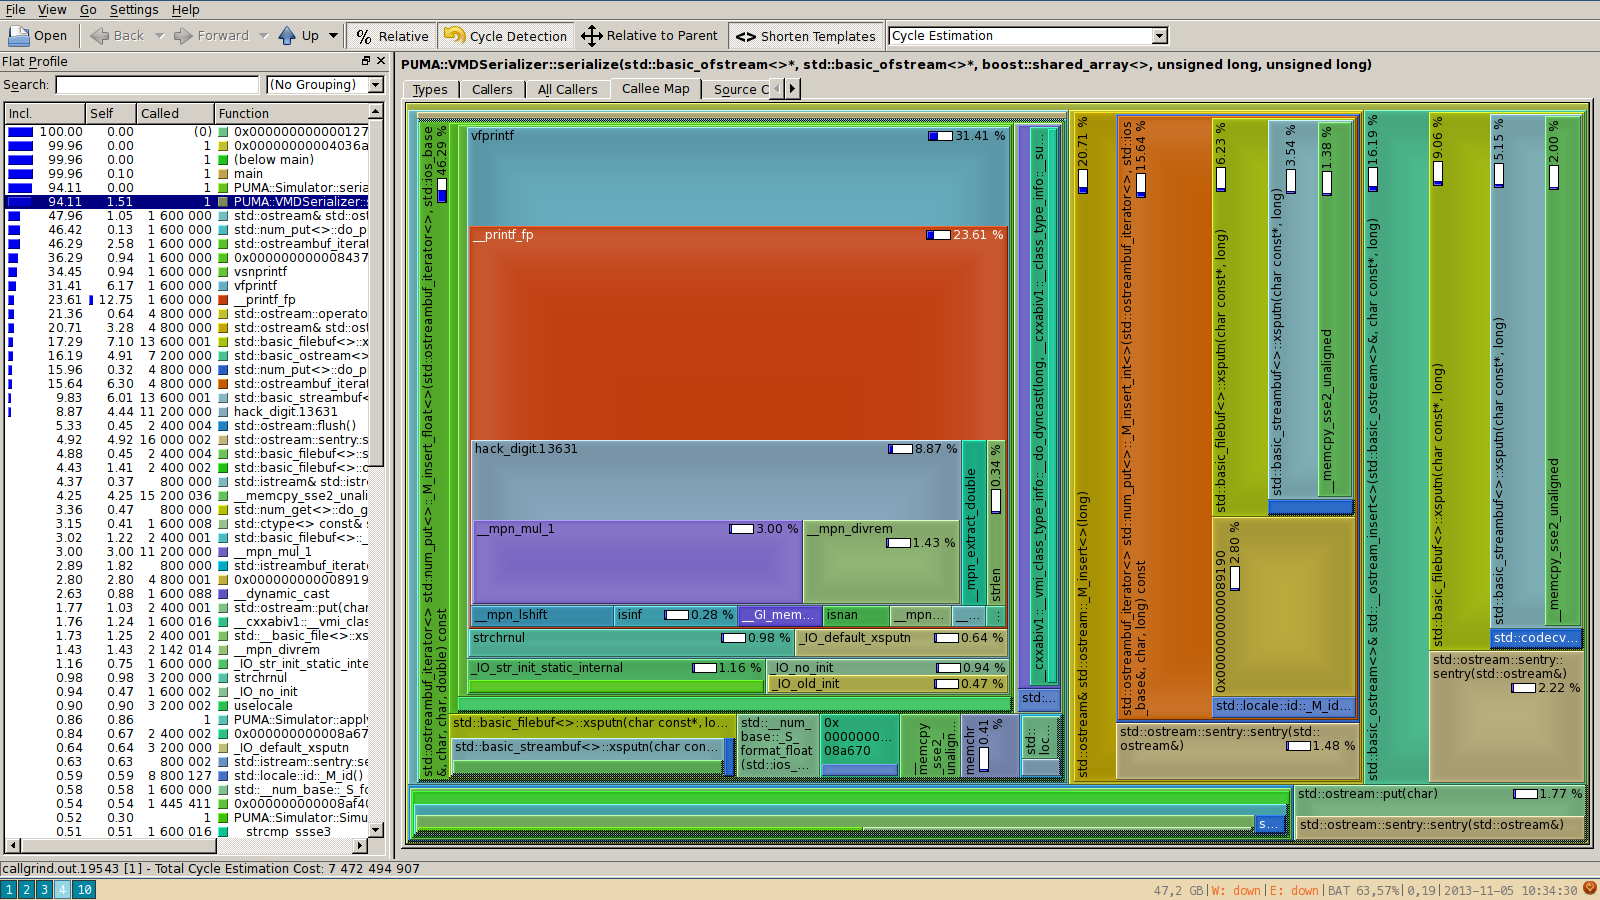
\includegraphics[width=\textwidth]{before_opti.png}
\caption{Output before optimization}
\label{fig:before}
\end{figure}
\vspace{-0.5cm}
\begin{figure}[H]
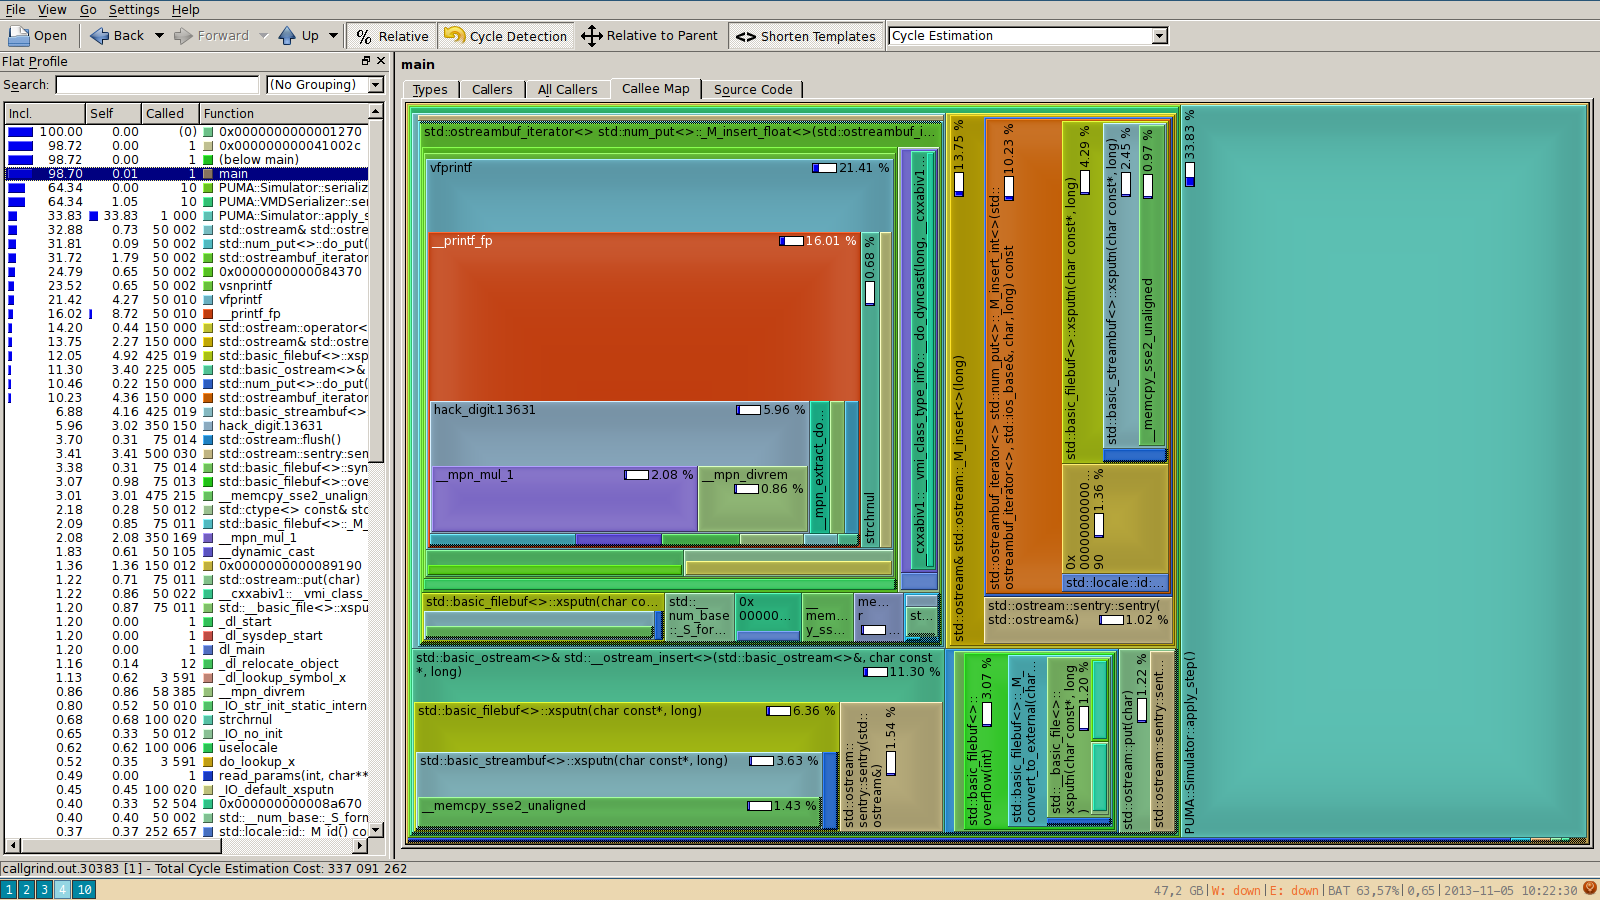
\includegraphics[width=\textwidth]{after_opti.png}
\caption{Output after optimization}
\label{fig:after}
\end{figure}

\newpage
\section{Links to Visualizations}\label{links}

This section includes online links to samples of each visualization type.  They are organized into the table below.  Note that all options are default unless specified otherwise.  

\begin{table}
\centering
\begin{tabular}{|l|l|l|l|l|}
\hline
\textbf{Type} & \textbf{Name} & \textbf{Map} & \textbf{Options} & \textbf{Link} \\ \hline
\multirow{3}{*}{\pbox{10cm}{\texttt{Visual} \\ \texttt{Molecular} \\ \texttt{Dynamics}}}
 & \emph{Unstable Hares} & \texttt{small.dat} & \texttt{dt=0.1} & \href{http://youtu.be/MmkpzO7vNhs}{youtu.be/MmkpzO7vNhs}  \\
 &  \emph{Stable Hares} & \texttt{small.dat} & \texttt{default} & \href{http://youtu.be/jbDyxL0PFB8}{youtu.be/jbDyxL0PFB8}\\
  &  \emph{Spiral Hares} & \texttt{spiral.dat} & \texttt{default}  & \href{http://youtu.be/sVR1NyPAj14}{youtu.be/sVR1NyPAj14}\\ \hline
\multirow{2}{*}{\pbox{10cm}{\texttt{Gnuplot}} }
 & \emph{Face hares} & \texttt{face.dat}& \texttt{default}   & \href{https://bazzle.me/animate.gif}{bazzle.me/animate.gif}\\
 & \emph{Face pumas} & \texttt{face.dat} & \texttt{default}  & \url{}\\ \hline
\multirow{3}{*}{\pbox{10cm}{\texttt{PPM}}} 
 & \emph{movie} &   \texttt{small.dat}& \texttt{default} & \href{https://bazzle.me/pumas/data/movie.gif}{bazzle.me/pumas/data/movie.gif} \\
 &   \emph{movie2}&  \texttt{small.dat}&\texttt{default}& \href{https://bazzle.me/pumas/data/movie2.gif}{bazzle.me/pumas/data/movie2.gif}\\
 &  \emph{movie3} & \texttt{islands.dat}& \texttt{default}&\href{https://bazzle.me/pumas/data/movie3.gif}{bazzle.me/pumas/data/movie3.gif} \\ \hline
 

\end{tabular}
\label{tb:parameters}
\end{table}


\end{appendices}

\end{document}


\bibliography{references}{}
\bibliographystyle{unsrt}


%TO DO
%  discretize equations
% reference the output visualization locations
% change parameters

